\chapter{Apprendimento Non Supervisionato e K-Means}
\begin{flushright}\small\textit{Lezione 8 -- 13/04/2026 -- G\'eron, Cap.\ 9}\end{flushright}

\section{Introduzione}

Nella maggior parte delle situazioni reali, i dati non arrivano con una ``risposta corretta'' o un'etichetta: la colonna target non esiste. In questi casi, possiamo affidarci all'\textbf{Apprendimento Non Supervisionato}, che studia come estrarre strutture e pattern intrinseci dai dati \emph{senza} una guida esterna.

\begin{notebox}[La metafora della torta di Yann LeCun]
Yann LeCun (Meta AI, Turing Award 2018): ``\emph{Se l'intelligenza fosse una torta, l'apprendimento non supervisionato sarebbe la torta, l'apprendimento supervisionato sarebbe la glassa e il Reinforcement Learning sarebbe la ciliegina.}''

La stragrande maggioranza dei dati disponibili nel mondo è \textbf{non etichettata}: si pensi a tutto il testo sul web, alle immagini di sorveglianza, ai log di sistema. Etichettare manualmente costa tempo e denaro.
\end{notebox}

\subsection{Applicazioni principali}

\begin{itemize}
    \item \textbf{Clustering}: raggruppare istanze simili -- segmentazione clienti, analisi immagini, sistemi di raccomandazione.
    \item \textbf{Rilevamento di anomalie} (\emph{anomaly detection}): identificare eventi rari o sospetti -- frodi bancarie, difetti di produzione, acquisti anomali.
    \item \textbf{Stima della densità}: stimare la distribuzione di probabilità dei dati -- usata a sua volta per l'anomaly detection.
    \item \textbf{Riduzione dimensionale}: PCA, t-SNE, UMAP, autoencoder -- comprimere le feature preservando l'informazione rilevante.
    \item \textbf{Apprendimento semi-supervisionato}: usare dati non etichettati per migliorare le prestazioni di modelli supervisionati quando le etichette sono poche.
\end{itemize}

\section{Classificazione vs.\ Clustering}

\begin{center}
\renewcommand{\arraystretch}{1.3}
\begin{tabular}{@{} l p{6.5cm} p{6.5cm} @{}}
\toprule
& \textbf{Classificazione (Supervisionata)} & \textbf{Clustering (Non supervisionato)} \\
\midrule
Etichette nel training & Sì (note a priori) & No \\
Classi & Definite prima del training & Emergono dai dati \\
Valutazione & Accuracy, F1, ROC-AUC & Inertia, Silhouette \\
Esempio & Iris: specie nota, si impara a distinguerla & Iris: nessuna specie, si trovano gruppi \\
\bottomrule
\end{tabular}
\end{center}

Il clustering \textbf{non} distingue i nomi delle classi a priori. È l'analista umano che, a posteriori, interpreta e dà un senso ai gruppi emersi. Considera il dataset Iris: a sinistra è un problema di classificazione (specie note), a destra è clustering (nessuna etichetta).

\begin{exbox}[Segmentazione clienti -- esempio tipico di clustering]
Un e-commerce raggruppa gli acquirenti in base ai prodotti acquistati e all'attività sul sito. L'algoritmo non sa che si tratta di ``giovani appassionati di tecnologia'' o ``adulti interessati al giardinaggio'' -- è l'analista che dà il nome al cluster. Una volta identificati, ogni segmento può ricevere campagne di marketing personalizzate.
\end{exbox}

\section{L'algoritmo K-Means}

Il \textbf{K-Means} è l'algoritmo di clustering più diffuso. Si basa sul concetto di \textbf{centroide}: il baricentro (centro di massa) di un cluster.

\subsection{Funzionamento passo per passo}

\begin{enumerate}
    \item \textbf{Inizializzazione}: si posizionano casualmente $k$ centroidi nello spazio dei dati.
    \item \textbf{Assegnazione}: ogni istanza viene assegnata al centroide più vicino sfruttando la distanza euclidea $d = \sum_{i} \sqrt{(x_C - x_i)^2 + (y_C - y_i)^2}$, dove $C$ è il centroide e $i$ sono i punti nella nuvola.
    \item \textbf{Aggiornamento}: ogni centroide viene spostato alla media delle istanze assegnate.
    \item \textbf{Ripetizione}: i passi 2--3 si ripetono finché i centroidi smettono di muoversi (\emph{convergenza}).
\end{enumerate}

\begin{center}
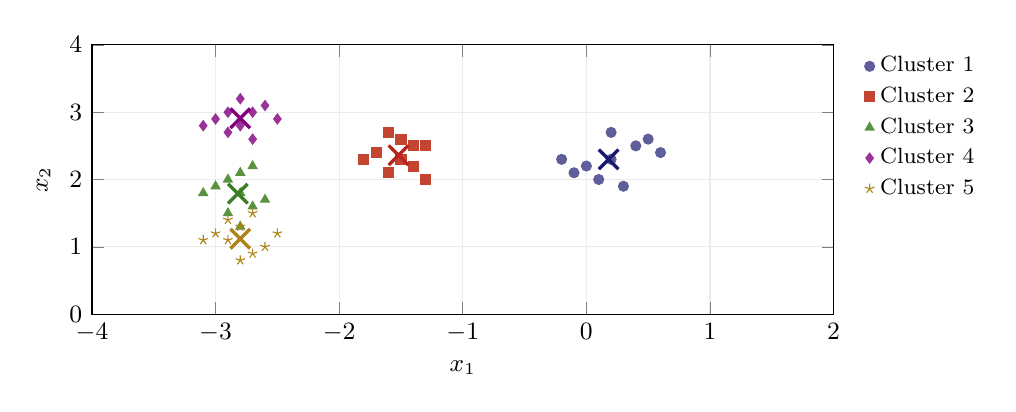
\begin{tikzpicture}[font=\small]
\begin{axis}[
    width=11cm, height=5cm,
    xlabel={$x_1$}, ylabel={$x_2$},
    xmin=-4, xmax=2, ymin=0, ymax=4,
    grid=major, grid style={gray!15},
    legend pos=outer north east,
    legend style={font=\footnotesize, cells={anchor=west},
                  legend columns=1, draw=none}
]
\addplot[only marks, mark=*, mark size=1.8pt, MidnightBlue!70]
    coordinates {
        (0.2,2.3)(0.1,2.0)(0.4,2.5)(0.3,1.9)(0.0,2.2)
        (0.5,2.6)(-0.1,2.1)(0.2,2.7)(0.6,2.4)(-0.2,2.3)
    };
\addlegendentry{Cluster 1}
\addplot[only marks, mark=square*, mark size=1.8pt, BrickRed!80]
    coordinates {
        (-1.5,2.3)(-1.6,2.1)(-1.4,2.5)(-1.3,2.0)(-1.7,2.4)
        (-1.5,2.6)(-1.6,2.7)(-1.4,2.2)(-1.8,2.3)(-1.3,2.5)
    };
\addlegendentry{Cluster 2}
\addplot[only marks, mark=triangle*, mark size=1.8pt, OliveGreen!80]
    coordinates {
        (-2.8,1.8)(-2.9,2.0)(-2.7,1.6)(-2.8,2.1)(-3.0,1.9)
        (-2.9,1.5)(-2.7,2.2)(-2.8,1.3)(-3.1,1.8)(-2.6,1.7)
    };
\addlegendentry{Cluster 3}
\addplot[only marks, mark=diamond*, mark size=1.8pt, Purple!80]
    coordinates {
        (-2.8,2.8)(-2.9,3.0)(-2.7,2.6)(-3.0,2.9)(-2.6,3.1)
        (-2.8,3.2)(-2.9,2.7)(-3.1,2.8)(-2.7,3.0)(-2.5,2.9)
    };
\addlegendentry{Cluster 4}
\addplot[only marks, mark=star, mark size=1.8pt, Goldenrod!80!black]
    coordinates {
        (-2.8,1.3)(-2.9,1.1)(-2.7,1.5)(-3.0,1.2)(-2.6,1.0)
        (-2.8,0.8)(-2.9,1.4)(-3.1,1.1)(-2.7,0.9)(-2.5,1.2)
    };
\addlegendentry{Cluster 5}
\addplot[mark=x, mark size=5pt, very thick, MidnightBlue] coordinates {(0.18, 2.3)};
\addplot[mark=x, mark size=5pt, very thick, BrickRed] coordinates {(-1.52, 2.36)};
\addplot[mark=x, mark size=5pt, very thick, OliveGreen] coordinates {(-2.82, 1.79)};
\addplot[mark=x, mark size=5pt, very thick, Purple] coordinates {(-2.8, 2.91)};
\addplot[mark=x, mark size=5pt, very thick, Goldenrod!80!black] coordinates {(-2.8, 1.12)};
\end{axis}
\end{tikzpicture}
\end{center}

La convergenza è \textbf{garantita matematicamente}: la somma delle distanze quadratiche tra ogni istanza e il suo centroide più vicino (\emph{inerzia}) può solo diminuire ad ogni iterazione e non può essere negativa -- quindi converge in un numero finito di passi. In pratica converge molto velocemente, spesso in poche iterazioni.

\subsection{Tassellazione di Voronoi}

Il risultato finale divide lo spazio in \textbf{regioni di Voronoi}: ogni punto dello spazio è più vicino al proprio centroide che a qualsiasi altro. I confini tra regioni adiacenti sono i \textbf{decision boundary} del modello.

\begin{notebox}[Robustezza di un cluster]
Un cluster è \textbf{robusto} se i suoi punti sono lontani dai confini della tassellazione. Se un nuovo punto cade lontano dal confine, la sua assegnazione è affidabile. Se cade vicino al confine, è difficile affermare con certezza a quale cluster appartenga -- ed è qui che il \emph{soft clustering} è più informativo dell'\emph{hard clustering}.
\end{notebox}

\subsection{Hard clustering vs.\ Soft clustering}

\begin{itemize}
    \item \textbf{Hard clustering} (default): ogni istanza appartiene a \emph{esattamente} un cluster.
    \item \textbf{Soft clustering}: si assegna a ogni istanza un \textbf{punteggio per ciascun cluster} -- la distanza dal centroide, oppure una probabilità. Più informativo, ma meno netto.
\end{itemize}

In Scikit-learn, \texttt{kmeans.transform(X\_new)} restituisce la distanza di ogni nuova istanza da ciascun centroide -- questo vettore di $k$ distanze può essere usato direttamente come vettore di feature per un modello downstream (\textbf{riduzione dimensionale non lineare}).

\section{Inizializzazione dei centroidi e K-Means++}

L'algoritmo non garantisce di trovare l'\textbf{ottimo globale}: se i centroidi iniziali sono sfortunati, si può convergere a una soluzione sub-ottimale. Ci sono due strategie principali per mitigare questo rischio.
Eseguire K-Means più volte con centroidi iniziali diversi e tenere la soluzione con l'\textbf{inerzia} (somma delle distanze quadratiche) più bassa.
Introdotto da Arthur \& Vassilvitskii (2006), seleziona i centroidi iniziali in modo che siano \textbf{distanti tra loro}:

\begin{enumerate}
    \item Scegliere il primo centroide $c^{(1)}$ casualmente tra le istanze.
    \item Per ogni istanza $x^{(i)}$, calcolare $D(x^{(i)})$ = distanza dal centroide già scelto più vicino.
    \item Scegliere il nuovo centroide $c^{(i)}$ con probabilità proporzionale a $D(x^{(i)})^2$: le istanze più lontane dai centroidi già scelti sono molto più probabili di essere scelte.
    \item Ripetere i passi 2--3 finché tutti i $k$ centroidi sono stati scelti.
\end{enumerate}

Questo fa sì che i centroidi iniziali siano ben distribuiti, riducendo drasticamente la probabilità di convergere a soluzioni sub-ottimali. \textbf{È il default di Scikit-learn}.


\subsection{Mini-Batch K-Means}

Per dataset molto grandi che non entrano in memoria, \texttt{MiniBatchKMeans} aggiorna i centroidi su \textbf{mini-batch} di istanze invece che sull'intero dataset. È circa 3--4 volte più veloce del K-Means standard, con un'inerzia leggermente superiore.

\section{Scegliere il numero ottimale di cluster $k$}

In un dataset reale (magari a 10 dimensioni) non è ovvio quanti centroidi creare. Si usano due metodi principali.

\subsection{Metodo del Gomito (Elbow Method)}

Si calcola l'\textbf{inerzia} per diversi valori di $k$ e si traccia la curva. L'inerzia \textbf{diminuisce sempre} all'aumentare di $k$ (più cluster $\to$ ogni punto è più vicino al proprio centroide). Si cerca il \textbf{punto di flesso} (il ``gomito'') dove la curva inizia ad appiattirsi.

\begin{center}
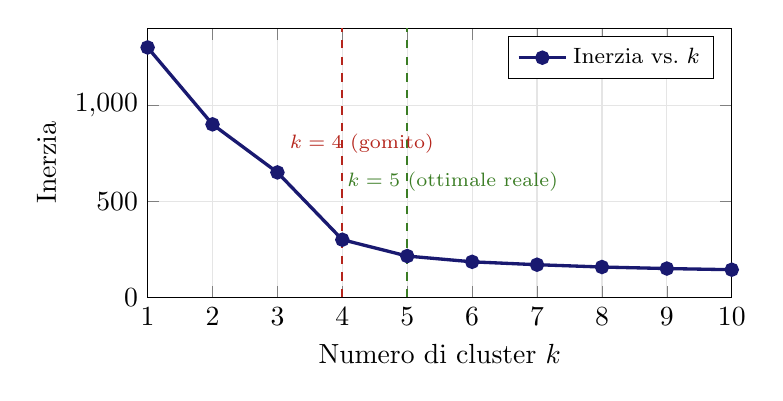
\begin{tikzpicture}
\begin{axis}[
    width=9cm, height=5cm,
    xlabel={Numero di cluster $k$},
    ylabel={Inerzia},
    xmin=1, xmax=10, ymin=0, ymax=1400,
    xtick={1,2,3,4,5,6,7,8,9,10},
    grid=major, grid style={gray!20},
    legend pos=north east,
    legend style={font=\footnotesize}
]
\addplot[very thick, MidnightBlue, mark=*] coordinates {
    (1,1300)(2,900)(3,650)(4,300)(5,215)(6,185)(7,170)(8,158)(9,150)(10,144)
};
\addlegendentry{Inerzia vs.\ $k$}
\addplot[thick, BrickRed, dashed] coordinates {(4,0)(4,1400)};
\addplot[thick, OliveGreen, dashed] coordinates {(5,0)(5,1400)};
\node[font=\scriptsize, BrickRed] at (axis cs:4.3, 800) {$k=4$ (gomito)};
\node[font=\scriptsize, OliveGreen] at (axis cs:5.7, 600) {$k=5$ (ottimale reale)};
\end{axis}
\end{tikzpicture}
\end{center}

\begin{warnbox}[Limite del metodo del gomito]
Il gomito è utile ma non sempre preciso: la curva può essere ``arrotondata'' senza un punto di flesso netto. Nel dataset a 5 blob, il gomito suggerisce $k=4$ ma il valore corretto è $k=5$. Serve sempre guardare anche il grafico dei dati e il coefficiente di Silhouette.
\end{warnbox}

\subsection{Coefficiente di Silhouette}

È una metrica più raffinata che valuta quanto ogni istanza è ben inserita nel proprio cluster. Per ogni istanza:
\begin{itemize}
    \item $a$ = distanza media dagli altri punti dello \emph{stesso} cluster (intra-cluster).
    \item $b$ = distanza media dai punti del \emph{cluster più vicino} (inter-cluster, il secondo più vicino).
\end{itemize}

\begin{equation}
s = \frac{b - a}{\max(a,\, b)}
\end{equation}

\begin{center}
\renewcommand{\arraystretch}{1.3}
\begin{tabular}{@{} c p{14cm} @{}}
\toprule
\textbf{Valore di $s$} & \textbf{Interpretazione} \\
\midrule
$s \approx +1$ & L'istanza è ben inserita nel suo cluster, lontana dagli altri -- ottima clusterizzazione. \\
$s \approx 0$ & L'istanza è vicina al confine tra due cluster -- assegnazione incerta. \\
$s < 0$ & $a > b$: l'istanza è stata assegnata al cluster sbagliato. \\
\bottomrule
\end{tabular}
\end{center}

Il \textbf{silhouette score} globale è la media dei coefficienti di tutte le istanze. Si calcola con \texttt{silhouette\_score(X, kmeans.labels\_)}.

\begin{center}
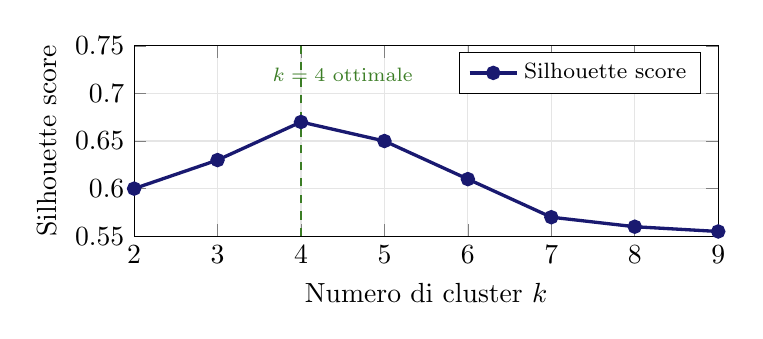
\begin{tikzpicture}
\begin{axis}[
    width=9cm, height=4cm,
    xlabel={Numero di cluster $k$},
    ylabel={Silhouette score},
    xmin=2, xmax=9, ymin=0.55, ymax=0.75,
    xtick={2,3,4,5,6,7,8,9},
    grid=major, grid style={gray!20},
    legend pos=north east,
    legend style={font=\footnotesize}
]
\addplot[very thick, MidnightBlue, mark=*] coordinates {
    (2,0.60)(3,0.63)(4,0.67)(5,0.65)(6,0.61)(7,0.57)(8,0.56)(9,0.555)
};
\addlegendentry{Silhouette score}
\addplot[thick, OliveGreen, dashed] coordinates {(4,0.55)(4,0.75)};
\node[font=\scriptsize, OliveGreen] at (axis cs:4.5, 0.72) {$k=4$ ottimale};
\end{axis}
\end{tikzpicture}
\end{center}

\subsection{Diagramma a coltello (Silhouette Diagram)}

Una visualizzazione ancora più informativa è il \textbf{silhouette diagram}: per ogni valore di $k$, si disegna un ``coltello'' per cluster. Ogni coltello mostra i coefficienti di silhouette ordinati in senso decrescente per tutte le istanze di quel cluster.

\begin{itemize}
    \item L'\textbf{altezza} del coltello indica il numero di istanze nel cluster.
    \item La \textbf{larghezza} rappresenta il valore del coefficiente (più largo = meglio).
    \item La \textbf{linea tratteggiata verticale} rossa indica la media globale. Un buon clustering ha tutte le lame che superano questa linea e hanno dimensioni simili.
\end{itemize}

\begin{center}
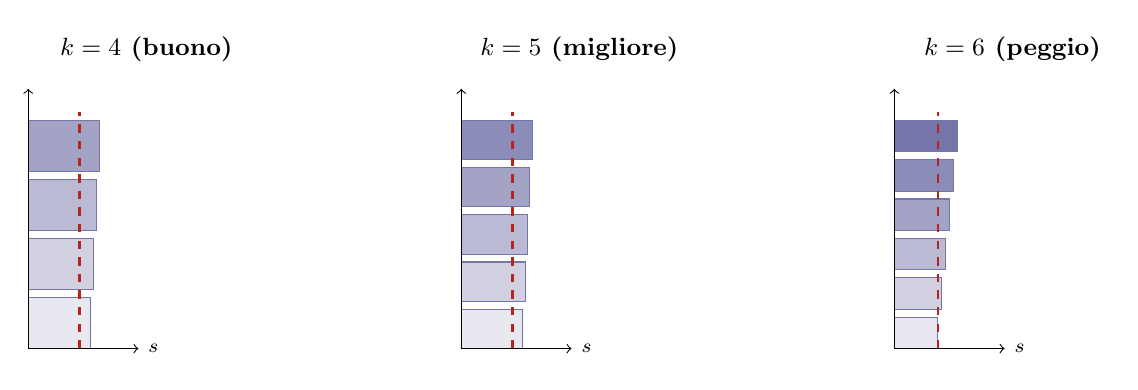
\begin{tikzpicture}[font=\scriptsize]
\foreach \k/\label in {4/{$k=4$ (buono)}, 5/{$k=5$ (migliore)}, 6/{$k=6$ (peggio)}} {
    \pgfmathsetmacro{\xshift}{(\k-4)*5.5}
    \begin{scope}[xshift=\xshift cm]
        \node[font=\small\bfseries] at (1.5, 3.8) {\label};
        \pgfmathsetmacro{\avgline}{(\k==4)?0.62:(\k==5)?0.65:0.55}
        \foreach \c in {1,...,\k} {
            \pgfmathsetmacro{\ystart}{(\c-1)*3.0/\k}
            \pgfmathsetmacro{\ystop}{\c*3.0/\k - 0.1}
            \pgfmathsetmacro{\width}{(\k==4)?0.8+0.2*\c/\k:(\k==5)?0.75+0.15*\c/\k:0.5+0.3*\c/\k}
            \fill[MidnightBlue!\c0!white, draw=MidnightBlue!60, thin]
                (0, \ystart) rectangle (\width, \ystop);
        }
        \draw[BrickRed, thick, dashed] (\avgline, 0) -- (\avgline, 3.0);
        \draw[->] (0,0) -- (1.4,0) node[right]{$s$};
        \draw[->] (0,0) -- (0,3.3);
    \end{scope}
}
\end{tikzpicture}
\end{center}

\begin{notebox}[Come leggere il diagramma a coltello]
Il clustering è \textbf{buono} se tutte le ``lame'' superano la linea rossa tratteggiata (media globale) e hanno dimensioni simili tra loro. Se alcune lame non raggiungono la media o sono molto più piccole delle altre, quei cluster sono ``cattivi''.

Nel dataset a 5 blob: con $k=4$, un cluster è molto più grande degli altri; con $k=5$, tutti i cluster hanno dimensioni simili e valori di silhouette elevati. Quindi $k=5$ è la scelta migliore, anche se il metodo del gomito suggeriva $k=4$.
\end{notebox}

\section{Applicazioni del K-Means}

\subsection{Segmentazione di immagini}

K-Means può ridurre il numero di colori di un'immagine raggruppando i pixel per colore simile (\emph{color segmentation}). Ogni pixel viene sostituito con il colore medio del suo cluster -- utile per sistemi di object detection che hanno bisogno di semplificare la scena.

\subsection{Apprendimento semi-supervisionato con K-Means}
Una delle applicazioni più potenti del clustering: estrarre \textbf{istanze rappresentative} da un dataset non etichettato per minimizzare il lavoro di etichettatura manuale.

\begin{exbox}[Digits dataset -- da 74.8\% a 90.9\% con soli 50 label]
\textbf{Scenario}: 1\,400 immagini di cifre (dataset Digits), ma solo 50 possono essere etichettate manualmente.

\textbf{Baseline} (50 istanze casuali): Logistic Regression ottiene \textbf{74.8\%} di accuratezza.

\textbf{Con K-Means}:
\begin{enumerate}
    \item Clusterizzare le 1\,400 immagini in 50 cluster.
    \item Per ogni cluster, trovare l'immagine più vicina al centroide (\emph{immagine rappresentativa}).
    \item Etichettare solo queste 50 immagini rappresentative.
    \item Addestrare Logistic Regression su 50 istanze rappresentative $\to$ \textbf{84.9\%}.
    \item \textbf{Propagare le etichette} a tutte le istanze dello stesso cluster $\to$ \textbf{89.4\%}.
    \item Eliminare l'1\% più lontano dal centroide (outlier) $\to$ \textbf{90.9\%}.
\end{enumerate}

Con soli 50 label (meno di 5 per cifra in media) si raggiunge la stessa accuratezza del modello addestrato sull'intero dataset etichettato (90.7\%). Le etichette propagate sono accurate al 97.5\%.
\end{exbox}

\section{Limiti del K-Means}

Nonostante sia veloce e scalabile, K-Means ha limiti importanti:

\begin{itemize}
    \item \textbf{Bisogna specificare $k$ a priori}: non sempre è ovvio quanti cluster ci sono.
    \item \textbf{Convergenza a ottimi locali}: l'inizializzazione conta; K-Means++ e \texttt{n\_init} riducono ma non eliminano il rischio.
    \item \textbf{Cluster sferici e isotropi}: K-Means lavora bene con ``bolle'' circolari (\texttt{make\_blobs}), ma fallisce con:
    \begin{itemize}
        \item cluster di \textbf{forma non sferica} (es.\ mezze lune, spirali -- \texttt{make\_moons});
        \item cluster di \textbf{densità o dimensioni diverse};
        \item cluster con \textbf{forma ellittica} orientata.
    \end{itemize}
    \item \textbf{Sensibile alla scala}: le feature non scalate distorcono le distanze. \textbf{Sempre scalare i dati prima di K-Means}.
\end{itemize}

\begin{center}
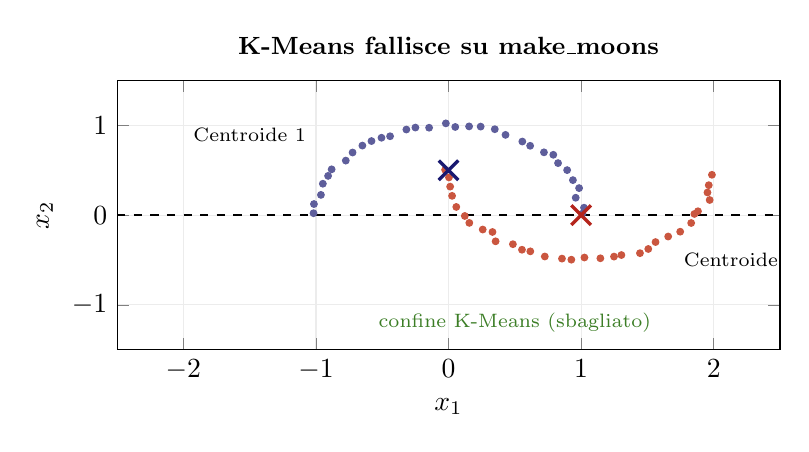
\begin{tikzpicture}
\begin{axis}[
    width=10cm, height=5cm,
    xlabel={$x_1$}, ylabel={$x_2$},
    xmin=-2.5, xmax=2.5, ymin=-1.5, ymax=1.5,
    grid=major, grid style={gray!15},
    title={K-Means fallisce su make\_moons},
    title style={font=\small\bfseries}
]
\foreach \a in {0,0.1,...,3.14} {
    \pgfmathsetmacro{\x}{cos(\a r) + 0.03*(rand)}
    \pgfmathsetmacro{\y}{sin(\a r) + 0.03*(rand)}
    \addplot[only marks, mark=*, mark size=1.2pt, MidnightBlue!70]
        coordinates {(\x, \y)};
}
\foreach \a in {0,0.1,...,3.14} {
    \pgfmathsetmacro{\x}{1 - cos(\a r) + 0.03*(rand)}
    \pgfmathsetmacro{\y}{0.5 - sin(\a r) + 0.03*(rand)}
    \addplot[only marks, mark=*, mark size=1.2pt, BrickRed!70]
        coordinates {(\x, \y)};
}
\addplot[only marks, mark=x, mark size=5pt, very thick, MidnightBlue]
    coordinates {(0.0, 0.5)};
\addplot[only marks, mark=x, mark size=5pt, very thick, BrickRed]
    coordinates {(1.0, 0.0)};
\node[font=\scriptsize] at (axis cs:-1.5, 0.9) {Centroide 1};
\node[font=\scriptsize] at (axis cs:2.2, -0.5) {Centroide 2};
\addplot[thick, black, dashed, domain=-2.5:2.5, samples=2] {0};
\node[font=\scriptsize, OliveGreen] at (axis cs:0.5, -1.2) {confine K-Means (sbagliato)};
\end{axis}
\end{tikzpicture}
\end{center}

\begin{notebox}[Non esiste una ``pallottola d'argento'']
Non esiste un algoritmo di clustering perfetto per ogni dataset. K-Means per le forme circolari, DBSCAN per le forme arbitrarie basate sulla densità (mezze lune, spirali), Gaussian Mixture Models per cluster ellissoidali. La scelta dipende dai dati.
\end{notebox}